\documentclass{beamer}
\usepackage[utf8]{inputenc}
\usepackage{graphicx}
\usepackage{listings}
\usepackage{xcolor}
\usepackage{tabularx}
\usepackage{tikz}
\usetikzlibrary{positioning, shapes.geometric, arrows}

\definecolor{primary}{RGB}{41, 128, 185}     
\definecolor{secondary}{RGB}{52, 152, 219}   
\definecolor{accent}{RGB}{231, 76, 60}      
\definecolor{success}{RGB}{46, 204, 113}     
\definecolor{warning}{RGB}{241, 196, 15}    
\definecolor{dark}{RGB}{44, 62, 80}          
\definecolor{light}{RGB}{236, 240, 241}      

\usetheme{Madrid}
\usecolortheme[named=primary]{structure}
\setbeamercolor{title}{fg=white}
\setbeamercolor{frametitle}{fg=white, bg=primary}
\setbeamercolor{block title}{fg=white, bg=secondary}
\setbeamercolor{block body}{fg=dark, bg=light!50}
\setbeamercolor{alerted text}{fg=accent}
\setbeamercolor{itemize item}{fg=primary}
\setbeamercolor{itemize subitem}{fg=secondary}
\setbeamercolor{enumerate item}{fg=primary}
\setbeamercolor{normal text}{fg=dark}

\setbeamertemplate{blocks}[rounded][shadow=true]


\subtitle{\color{secondary}Real-time Academic Sentiment Hub \& Resource Management}
\date{\color{dark}January 2026}
\institute{\color{dark}Smart Tutor Development Team}

\begin{document}

\begin{frame}
    \begin{tikzpicture}[remember picture,overlay]
        \fill[primary] (current page.north west) rectangle (current page.south east);
        \node[white, font=\Huge, align=center, text width=0.8\paperwidth] at (current page.center) {
            \textbf{Smart Tutor} \\[5pt]

        };
        \node[white, align=center, yshift=-2cm] at (current page.center) {
            Real-time Academic Sentiment Hub \& Resource Management \\[10pt]
            \small Kwtee ngnouba junior rayan    ictu20241377\\
             \small  Izuchuku chijioke emmanuel  Ictu20241760\\ 
             \Small Supervisor: Eng Tekoh Palma\\ 
       
        };
    \end{tikzpicture}
\end{frame}

\begin{frame}{Project Overview}
    \begin{columns}
        \column{0.5\textwidth}
        \begin{alertblock}{Problem Statement}
            \color{accent}\textbf{Traditional learning platforms lack real-time feedback loops between students and teachers.}
        \end{alertblock}
        
        \begin{exampleblock}{Our Solution}
            \color{success}\textbf{A dual-purpose educational platform:}
            \begin{itemize}
                \item \textbf{Sentiment Hub:} \textcolor{secondary}{Real-time misunderstanding reporting}
                \item \textbf{Admin PDF Control:} \textcolor{secondary}{Secure, high-performance resource management}
            \end{itemize}
        \end{exampleblock}
        
        \column{0.5\textwidth}
        \begin{figure}
            \centering
            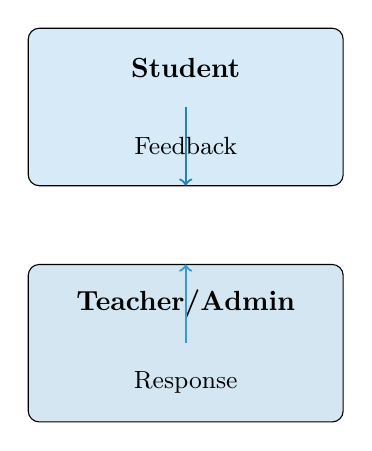
\begin{tikzpicture}
                \draw[fill=secondary!20, rounded corners] (0,0) rectangle (4,2);
                \node at (2,1.5) {\textbf{Student}};
                \draw[->, thick, primary] (2,1) -- (2,0);
                \node at (2,0.5) {\small Feedback};
                
                \draw[fill=primary!20, rounded corners] (0,-3) rectangle (4,-1);
                \node at (2,-1.5) {\textbf{Teacher/Admin}};
                \draw[->, thick, secondary] (2,-2) -- (2,-1);
                \node at (2,-2.5) {\small Response};
            \end{tikzpicture}
            \caption{Real-time Communication Flow}
        \end{figure}
    \end{columns}
\end{frame}

\begin{frame}{Software Requirements (SRS)}
    \begin{columns}
        \column{0.5\textwidth}
        \begin{block}{Student Requirements \color{success}\checkmark}
            \begin{itemize}
                \item \textbf{\textcolor{primary}{Access}} to curated PDF materials
                \item \textbf{\textcolor{primary}{Post}} real-time inquiries/sentiments
                \item \textbf{\textcolor{primary}{View}} teacher responses
                \item \textbf{\textcolor{primary}{Dashboard}} for activity tracking
            \end{itemize}
        \end{block}
        
        \column{0.5\textwidth}
        \begin{block}{Admin Requirements \color{success}\checkmark}
            \begin{itemize}
                \item \textbf{\textcolor{accent}{Full CRUD}} control over resources
                \item \textbf{\textcolor{accent}{Secure file deletion}} on VPS
                \item \textbf{\textcolor{accent}{User/role}} management
                \item \textbf{\textcolor{accent}{Analytics}} and monitoring
            \end{itemize}
        \end{block}
    \end{columns}
    
    \vspace{0.5cm}
    \begin{alertblock}{Non-Functional Requirements}
        \centering
        \begin{tabular}{|c|c|}
            \hline
            \rowcolor{primary!20}
            \textbf{Criteria} & \textbf{Target} \\
            \hline
            Performance & 1000 concurrent users, <2s response \\
            \hline
            Availability & 99.5\% uptime \\
            \hline
            Security & TLS 1.2+, encrypted data \\
            \hline
            Scalability & Horizontal scaling ready \\
            \hline
        \end{tabular}
    \end{alertblock}
\end{frame}

\begin{frame}{System Architecture}
    \centering
    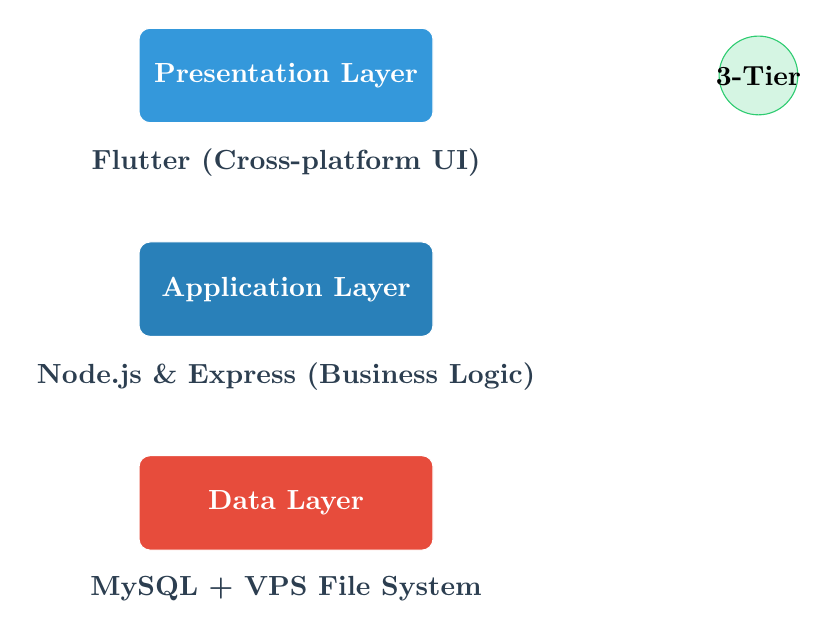
\begin{tikzpicture}[
        node distance=1.5cm,
        layer/.style={rectangle, rounded corners, draw=white, fill=#1, text=white, text width=3.5cm, text centered, minimum height=1.2cm, font=\bfseries},
        arrow/.style={->, >=stealth, thick, white}
    ]

        \node (presentation) [layer=secondary] {Presentation Layer};
        \node (application) [layer=primary, below=of presentation] {Application Layer};
        \node (data) [layer=accent, below=of application] {Data Layer};
    
        \draw[arrow] (presentation) -- (application);
        \draw[arrow] (application) -- (data);
        
        \node[below=0.2cm of presentation, text=dark] {\textbf{Flutter (Cross-platform UI)}};
        \node[below=0.2cm of application, text=dark] {\textbf{Node.js \& Express (Business Logic)}};
        \node[below=0.2cm of data, text=dark] {\textbf{MySQL + VPS File System}};
        

        \draw[fill=success!20, draw=success] (6,0) circle (0.5);
        \node at (6,0) {\textbf{3-Tier}};
    \end{tikzpicture}
    
    \vspace{0.5cm}
    \begin{block}{Architecture Pattern}
        \centering
        \textbf{\textcolor{primary}{Three-Tier Architecture}} with clear separation of concerns
    \end{block}
\end{frame}

\begin{frame}{Behavioral Design (Use Case)}
    \begin{columns}
        \column{0.45\textwidth}
        \begin{block}{\textcolor{secondary}{Student Interactions}}
            \begin{enumerate}
                \item \textbf{Login/Register}
                \item \textbf{Browse PDF Resources}
                \item \textbf{Post Sentiment/Question}
                \item \textbf{View Responses}
                \item \textbf{Track Progress}
            \end{enumerate}
        \end{block}
        
        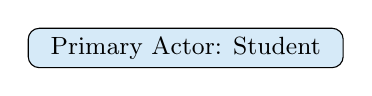
\begin{tikzpicture}
            \draw[fill=secondary!20, rounded corners] (0,0) rectangle (4,0.5);
            \node at (2,0.25) {\small Primary Actor: Student};
        \end{tikzpicture}
        
        \column{0.45\textwidth}
        \begin{block}{\textcolor{accent}{Admin Interactions}}
            \begin{enumerate}
                \item \textbf{Upload PDF Resources}
                \item \textbf{Delete/Update Materials}
                \item \textbf{Monitor Sentiment Hub}
                \item \textbf{Respond to Students}
                \item \textbf{System Analytics}
            \end{enumerate}
        \end{block}
        
        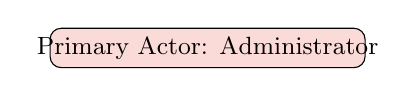
\begin{tikzpicture}
            \draw[fill=accent!20, rounded corners] (0,0) rectangle (4,0.5);
            \node at (2,0.25) {\small Primary Actor: Administrator};
        \end{tikzpicture}
    \end{columns}
    
    \vspace{0.5cm}
    \centering
    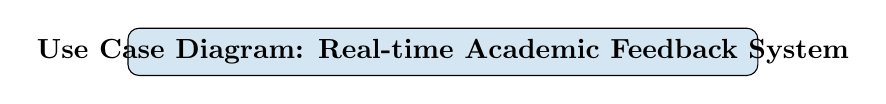
\begin{tikzpicture}
        \draw[fill=primary!20, rounded corners] (0,0) rectangle (8,0.6);
        \node at (4,0.3) {\textbf{Use Case Diagram: Real-time Academic Feedback System}};
    \end{tikzpicture}
\end{frame}

\begin{frame}{Structural Design (Class Diagram)}
    \centering
    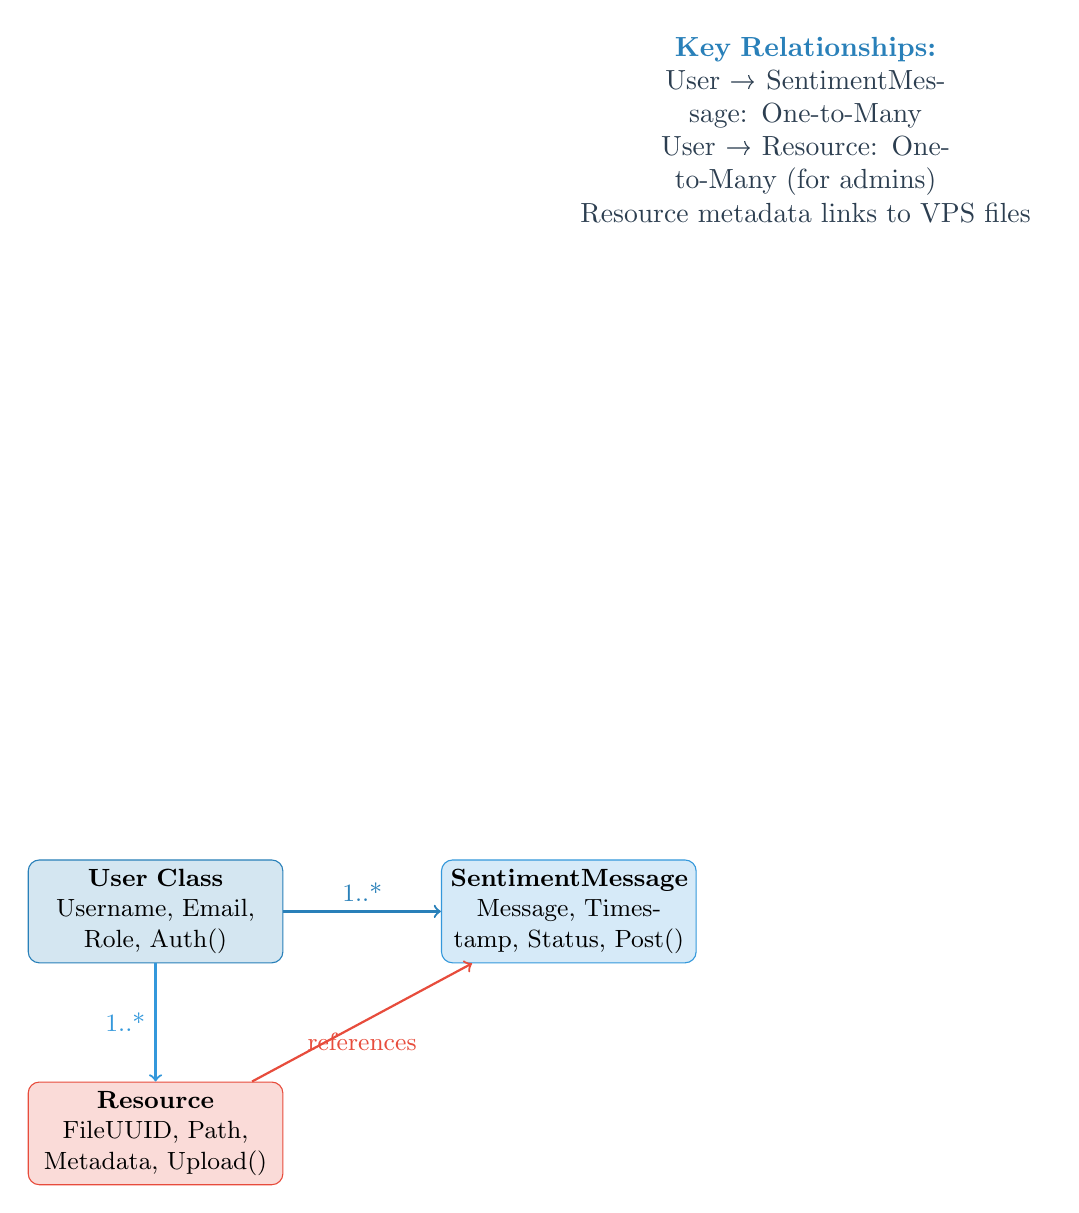
\begin{tikzpicture}[
        class/.style={rectangle, draw=#1, fill=#1!20, text width=3cm, minimum height=1cm, text centered, rounded corners, font=\small}
    ]

        \node (user) [class=primary] {\textbf{User Class}\\\small Username, Email, Role, Auth()};
        \node (sentiment) [class=secondary, right=2cm of user] {\textbf{SentimentMessage}\\\small Message, Timestamp, Status, Post()};
        \node (resource) [class=accent, below=1.5cm of user] {\textbf{Resource}\\\small FileUUID, Path, Metadata, Upload()};
        
        \draw[->, thick, primary] (user) -- node[above] {\small 1..*} (sentiment);
        \draw[->, thick, secondary] (user) -- node[left] {\small 1..*} (resource);
        \draw[->, thick, accent] (resource) -- node[below] {\small references} (sentiment);
        

        \node[text width=6cm, align=center, yshift=-1.5cm] at (current page.center) {
            \textbf{\textcolor{primary}{Key Relationships:}}\\
            \textcolor{dark}{User → SentimentMessage: One-to-Many}\\
            \textcolor{dark}{User → Resource: One-to-Many (for admins)}\\
            \textcolor{dark}{Resource metadata links to VPS files}
        };
    \end{tikzpicture}
\end{frame}

\begin{frame}{Data Design (Entity Relationship Diagram)}
    \begin{columns}
        \column{0.6\textwidth}
        \centering
        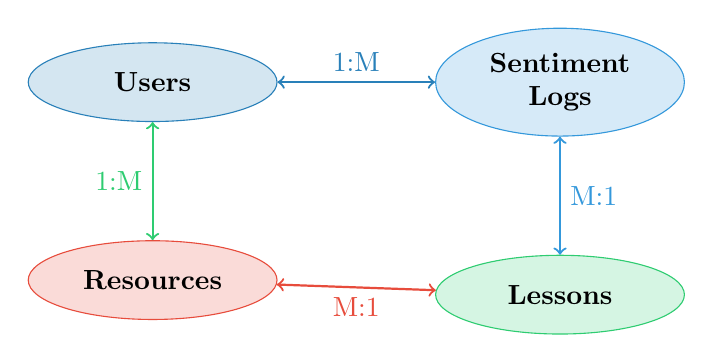
\begin{tikzpicture}[
            entity/.style={ellipse, draw=#1, fill=#1!20, text width=2cm, minimum height=1cm, text centered}
        ]
            \node (user) [entity=primary] {\textbf{Users}};
            \node (sentiment) [entity=secondary, right=2cm of user] {\textbf{Sentiment Logs}};
            \node (resource) [entity=accent, below=1.5cm of user] {\textbf{Resources}};
            \node (lesson) [entity=success, below=1.5cm of sentiment] {\textbf{Lessons}};
            

            \draw[<->, thick, primary] (user) -- node[above] {1:M} (sentiment);
            \draw[<->, thick, secondary] (sentiment) -- node[right] {M:1} (lesson);
            \draw[<->, thick, accent] (resource) -- node[below] {M:1} (lesson);
            \draw[<->, thick, success] (user) -- node[left] {1:M} (resource);
        \end{tikzpicture}
        
        \column{0.4\textwidth}
        \begin{block}{\textcolor{primary}{Database Design}}
            \begin{itemize}
                \item \textbf{\textcolor{secondary}{Normalization:}} 3rd Normal Form (3NF)
                \item \textbf{\textcolor{secondary}{Relationships:}} One-to-Many patterns
                \item \textbf{\textcolor{secondary}{Storage:}} DB stores metadata, VPS stores binaries
                \item \textbf{\textcolor{secondary}{Indexing:}} Optimized for frequent queries
            \end{itemize}
        \end{block}
    \end{columns}
    
    \vspace{0.3cm}
    \begin{alertblock}{Storage Strategy}
        \centering
        \textbf{Hybrid Approach:} Database stores \textcolor{accent}{"File Pointers" (UUIDs)} while VPS stores \textcolor{accent}{actual binary files}
    \end{alertblock}
\end{frame}

\begin{frame}{Agile Methodology (Scrum)}
    \centering
    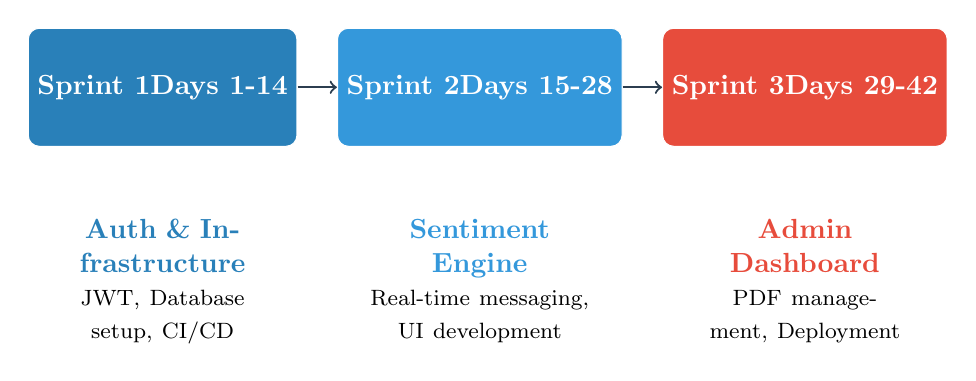
\begin{tikzpicture}[
        sprint/.style={rectangle, draw=white, fill=#1, text=white, rounded corners, minimum width=3cm, minimum height=1.5cm, text centered, font=\bfseries}
    ]
    
        \node (sprint1) [sprint=primary] {Sprint 1 \\ Days 1-14};
        \node (sprint2) [sprint=secondary, right=0.5cm of sprint1] {Sprint 2 \\ Days 15-28};
        \node (sprint3) [sprint=accent, right=0.5cm of sprint2] {Sprint 3 \\ Days 29-42};

        \draw[->, thick, dark] (sprint1) -- (sprint2);
        \draw[->, thick, dark] (sprint2) -- (sprint3);
        

        \node[below=0.8cm of sprint1, text width=3cm, align=center] {
            \textbf{\textcolor{primary}{Auth \& Infrastructure}}\\
            \footnotesize JWT, Database setup, CI/CD
        };
        \node[below=0.8cm of sprint2, text width=3cm, align=center] {
            \textbf{\textcolor{secondary}{Sentiment Engine}}\\
            \footnotesize Real-time messaging, UI development
        };
        \node[below=0.8cm of sprint3, text width=3cm, align=center] {
            \textbf{\textcolor{accent}{Admin Dashboard}}\\
            \footnotesize PDF management, Deployment
        };
    \end{tikzpicture}
    
    \vspace{0.8cm}
    \begin{columns}
        \column{0.5\textwidth}
        \begin{exampleblock}{Sprint Metrics}
            \centering
            \begin{tabular}{|c|c|}
                \hline
                \rowcolor{primary!20}
                \textbf{Metric} & \textbf{Value} \\
                \hline
                Velocity & 29 points/sprint \\
                \hline
                Test Coverage & 92\% \\
                \hline
                Bugs Reported & 8 \\
                \hline
                Team Satisfaction & 4.5/5 \\
                \hline
            \end{tabular}
        \end{exampleblock}
        
        \column{0.5\textwidth}
        \begin{alertblock}{Framework}
            \centering
            \textbf{\textcolor{accent}{Scrum Framework}}\\
            \small 3 Sprints × 14 days each
        \end{alertblock}
    \end{columns}
\end{frame}

\begin{frame}{Technical Implementation \& DevOps}
    \begin{columns}
        \column{0.33\textwidth}
        \begin{block}{\textcolor{primary}{Security}}
            \begin{itemize}
                \item \textbf{JWT Authentication}
                \item \textbf{Bcrypt Hashing} (salt rounds=12)
                \item \textbf{RBAC} (Role-Based Access)
                \item \textbf{HTTPS} Enforcement
                \item \textbf{Input Validation}
            \end{itemize}
        \end{block}
        
        \column{0.33\textwidth}
        \begin{block}{\textcolor{secondary}{Deployment}}
            \begin{itemize}
                \item \textbf{Ubuntu 22.04 LTS}
                \item \textbf{Nginx Reverse Proxy}
                \item \textbf{PM2 Process Manager}
                \item \textbf{Automated Scripts}
                \item \textbf{Health Monitoring}
            \end{itemize}
        \end{block}
        
        \column{0.33\textwidth}
        \begin{block}{\textcolor{accent}{Reliability}}
            \begin{itemize}
                \item \textbf{99.5\% Uptime}
                \item \textbf{Auto-restart}
                \item \textbf{Daily Backups}
                \item \textbf{Load Balancing}
                \item \textbf{Error Tracking}
            \end{itemize}
        \end{block}
    \end{columns}
    
    \vspace{0.5cm}
    \centering
    
\begin{tikzpicture}
        \draw[fill=success!20, rounded corners] (0,0) rectangle (10,0.6);
        \node at (5,0.3) {\textbf{Technology Stack: Flutter | Node.js | Express | MySQL | VPS}};
    \end{tikzpicture}
\end{frame}


\begin{frame}{Conclusion \& Future Scope}
    \begin{columns}
        \column{0.5\textwidth}
        \begin{block}{\textcolor{success}{Project Summary}}
            \textbf{Successfully delivered:}
            \begin{itemize}
                \item Scalable 3-tier architecture
                \item Real-time sentiment communication
                \item Secure PDF management system
                \item High test coverage (92\%)
                \item Agile delivery on time
            \end{itemize}
        \end{block}
        
        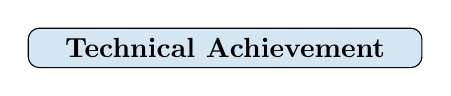
\begin{tikzpicture}
            \draw[fill=primary!20, rounded corners] (0,0) rectangle (5,0.5);
            \node at (2.5,0.25) {\textbf{Technical Achievement}};
        \end{tikzpicture}
        
        \column{0.5\textwidth}
        \begin{alertblock}{\textcolor{accent}{Future Work}}
            \textbf{Short-term (3 months):}
            \begin{itemize}
                \item \textcolor{secondary}{AI-powered sentiment analysis}
                \item \textcolor{secondary}{WebSockets for instant chat}
                \item \textcolor{secondary}{Advanced search capabilities}
                \item \textcolor{secondary}{Push notifications}
            \end{itemize}
            
            \textbf{Long-term (12 months):}
            \begin{itemize}
                \item \textcolor{secondary}{Multi-language support}
                \item \textcolor{secondary}{LMS integrations}
                \item \textcolor{secondary}{Predictive analytics}
            \end{itemize}
        \end{alertblock}
    \end{columns}
    
    \vspace{0.5cm}
    \centering
    \begin{exampleblock}{Final Remarks}
        \centering
        \textbf{Smart Tutor demonstrates modern software engineering practices in EdTech,}\\
        \textbf{combining cutting-edge technologies with user-centered design.}
    \end{exampleblock}
\end{frame}

\begin{frame}
    \begin{tikzpicture}[remember picture,overlay]
        \fill[primary] (current page.north west) rectangle (current page.south east);
        
        \foreach \i in {1,...,20} {
            \draw[white, opacity=0.1] (rand*12, rand*9) circle (0.3);
        }
        
        \node[white, font=\Huge, align=center] at (current page.center) {
            \textbf{Thank You!} \\[20pt]
            \Huge \textbf{Q \& A} \\[30pt]
            \small Smart Tutor Development Team \\[5pt]
        
        };
        
        \node[white, align=center, yshift=-3cm] at (current page.center) {
            \small \textbf{Contact:} kwetejunior9@gmail.com \\
            \small \textbf{GitHub:} https://github.com/Suraku237/smart-tutor \\
            \small \textbf{wesite:} http://smarttutor.duckdns.org/
        };
    \end{tikzpicture}
\end{frame}

\end{document}